\documentclass[12pt, notitlepage]{report}

\usepackage{geometry}
\usepackage{polski}
\usepackage[utf8]{inputenc}
\usepackage[T1]{fontenc}
\usepackage{enumitem}
\usepackage{graphicx}

\usepackage{etoolbox}
\makeatletter
\patchcmd{\chapter}{\if@openright\cleardoublepage\else\clearpage\fi}{}{}{}
\makeatother

\usepackage[toc]{appendix}
\renewcommand{\appendixtocname}{Dodatki}

\usepackage[
    backend=biber,
    style=alphabetic,
    sorting=ynt
    ]{biblatex}

\addbibresource{doc.bib}
\geometry{legalpaper, margin=0.8in}

\begin{document}

    \begin{titlepage}
        \thispagestyle{empty}
        \title{\Huge Zastosowania informatyki w medycynie \\[1cm]\Huge Automatyczne rozpoznawanie faz snu na podstawie diagramów EEG}
        \author{Szymon Bagiński \\[1cm]{\small Prowadzący: Dr hab. inż. Robert Burduk}}
        % \author{Szymon Bagiński\thanks{funded by the ShareLaTeX team}}
        \date{Czerwiec 2018}
        \maketitle
        \vfill
        \renewcommand{\chapter}[2]{}
        \begin{center}
            \Large \bfseries\contentsname
        \end{center}
        \tableofcontents
        \vfill
    \end{titlepage}    

    \chapter*{Wstęp}
    \addcontentsline{toc}{chapter}{Wstęp}
        Celem projektu było stworzenie programistycznej metody automatycznego rozpoznawania faz snu człowieka na podstawie zapisu sygnału elektroencefalograficznego (\textit{EEG}). Częścią zadania nie było opracowanie metody gromadzenia zapisów ani wykonywanie pomiarów sygnału. Zdecydowano się skorzystać z bazy danych dostępnej pod adresem \url{https://www.physionet.org/physiobank/database/sleep-edfx/}, udostępniającej pliki w formacie \textit{EDF} (European Data Format). 

        Z uwagi na brak wiedzy dziedzinowej, przy klasyfikacji zdecydowano się na zastosowanie sztucznej sieci neuronowej zamiast analitycznego podejścia do problemu. Przy implementacji sieci skorzystano z otwartoźródłowej biblioteki programistycznej \textit{TensorFlow}. Wykorzystano wersję biblioteki wykorzystującą technologię \textit{CUDA}, dzięki czemu skrócono czas uczenia sieci poprzez przeniesienie wielu równoległych obliczeń na kartę graficzną.

        Do wykonania skryptów wczytujących i przygotowujących dane, oraz do uczenia maszynowego został użyty język programowania \textit{Python}. Szczególnie przydatne okazały się pakiety:
        \begin{itemize}
            \item NumPy - obsługa danych tablicowych,
            \item PyEDFlib - obsługa plików \textit{EDF},
            \item PyWavelets - przetwarzania sygnału, Dyskretna Transformata Falkowa,
            \item TensorFlow - interfejs biblioteki do języka \textit{Python}.
        \end{itemize}

        Wszystkie skrypty, które powstały w ramach projektu można znaleźć w publicznym repozytorium pod adresem \url{www}. % TODO repo

    \chapter{Pozyskanie danych}
        Użyte w projekcie dane zostały pobrane ze strony internetowej \cite{}. Wykorzystane zapisy uzyskano w latach 1987-1991 podczas badań nad wpływem wieku na sen. Rekordy pochodzą od osób rasy kaukaskiej w wieku od 25 do 101 lat , które nie przyjmowały żadnych leków związanych ze snem. Sygnały były próbkowane z częstotliwością 100 Hz, a ich klasyfikacja została przeprowadzona przy pomocy reguł Rechtschaffen'a i Kales'a na bazie trzydziestosekundowych segmentów z kanałów \textit{Fpz-Cz} i \textit{Pz-Oz}. Każdy z segmentów został sklasyfikowany jako: przebudzony, nie-REM1, nie-REM2, nie-REM3, REM, niewielka aktywność, poruszenie lub nieokreślony.
        W tym projekcie został użyty jednak tylko kanał \textit{Pz-Oz}, a rozpoznawanymi fazami były: przebudzony, nie-REM1 + REM, nie-REM2, nie-REM3 + niewielka aktywność.
        Dokładny opis przebiegu badań znajduje się stronie internetowej bazy danych.
        
        Do trenowania sztucznej sieci neuronowej zostało wykorzystanych dwadzieścia siedem ponad dwudziestogodzinnych zapisów \textit{EEG}, a skuteczność klasyfikacji sprawdzono przy pomocy pięciu rekordów nie użytych przy trenowaniu. Obie listy plików znajdują się w dodatku \ref{appendix:A} i \ref{appendix:B}.

        \newpage

        \section{Wczytywanie danych z pliku EDF}
            W module \textit{EdfFile.py} została stworzona klasa \textit{EdfFile}, która jako argument konstruktora przyjmuje ścieżkę do pliku z elektroencefalogramem oraz ścieżkę do pliku, w którym znajdują się adnotacje.
            
            W funkcji \textit{\_\_init\_\_} zostało wykorzystanych kilka funkcjonalności z biblioteki PyEDFlib. Funkcja \textit{EdfReader} służy do odczytania danych z pliku i zwraca obiekt go reprezentujący, przez który mamy dostęp do właściwości zapisu takich jak między innymi:
            \begin{itemize}
                \item liczba sygnałów (kanałów) w pliku,
                \item lista etykiet sygnałów,
                \item wartości napięcia dla zczytanych próbek,
                \item lista częstotliwości sygnałów,
                \item lista adnotacji do faz snu,
                \item lista czasów przejść między fazami snu.                
            \end{itemize}
            W tym miejscu jest tworzona także kolekcja obiektów typu \textit{Signal}, które są "opakowaniem" na sygnały obecne w pliku.

            W klasie \textit{EdfFile} znajdują się także dwie funkcje odpowiedzialne za przygotowanie danych dla sieci neuronowej. Są to \textit{createOutput} oraz \textit{createInput}. Zwracają one dane odczytane z pliku w postaci macierzy, które następnie w skrypcie \textit{prepare.py} są agregowane. Tutaj także, ma miejsce kontrola poprawności danych i usunięcie błędnych próbek, aby nie umieszczać ich na wejściu sieci.

        \section{Przetwarzanie wstępne}
            Klasa \textit{Signal} posiada tylko jedną metodę. Jest nią \textit{getEpochs}, która dzieli sygnał na trzydziestosekundowe segmenty, tworzy odpowiadające im obiekty typu \textit{Epoch} i zwraca je w liście.
            Następnie, w skrypcie \textit{prepare.py} otrzymane w ten sposób obiekty są przekazywane do metody \textit{createOutput} i \textit{createInput} z klasy \textit{EdfFile}. Na każdym segmencie wywoływana jest metoda \textit{extractFeatures}, której zadaniem jest wyekstrahowanie dwunastu cech, które posłużą jako pobudzenia wejść sieci neuronowej.

    \chapter{Wyekstrahowanie cech z sygnału EEG}
        Wszystkie cechy zostały pozyskane przy użyciu Dyskretnej Transformaty Falkowej (DWPT - Discrete Wavelet Transform). Jest to przekształcenie podobne do transformaty Fouriera. Główna różnica polega na użyciu innego jądra przekształcenia. W transformacie Fouriera jądrem jest funkcja sinusoidalna, która w dziedzinie czasu jest nieograniczona, a w dziedzinie częstotliwości jest punktem. To zapewnia jej idealną rozdzielczość w dziedzinie częstotliwości natomiast czyni ją nieprzydatną w kontekście analizy czasowej. Ponieważ nośniki falek jak i ich widm nie są punktowe, analiza przy pomocy transformaty falkowej nie posiada idealnej rozdzielczości, ani w dziedzinie czasu ani w dziedzinie częstotliwości (następstwo zasady nieoznaczoności). transformata falkowa służy więc do analizy sygnałów niestacjonarnych, ponieważ dostarcza informacji o czasowo-częstotliwościowych zmianach sygnałów.

        W projekcie została użyta Dyskretna transformata pakietów falkowych (DWPT - Discrete wavelet packet transform), która jest rozszerzeniem Transformaty Falkowej. Dzieli ona oryginalny sygnał na dwie części: wysokie i niskie częstotliwości. Transformata falkowa rozkłada tylko niskie częstotliwości dokładnie, a DWPT to jej uogólniona wersja, która również rozkłada pasma wysokiej częstotliwości i prowadzi do powstania kompletnego drzewa pakietów falkowych (rysunek \ref{fig:tree}).

        W tym przypadku została użyta DWPT z falką Daubechies rzędu pierwszego do głębokości poziomu siódmego. Skorzystano z gotowej funkcjonalności biblioteki PyWavelets - WaveletPacket. 
            
        \begin{figure}[h!]
            \centering
            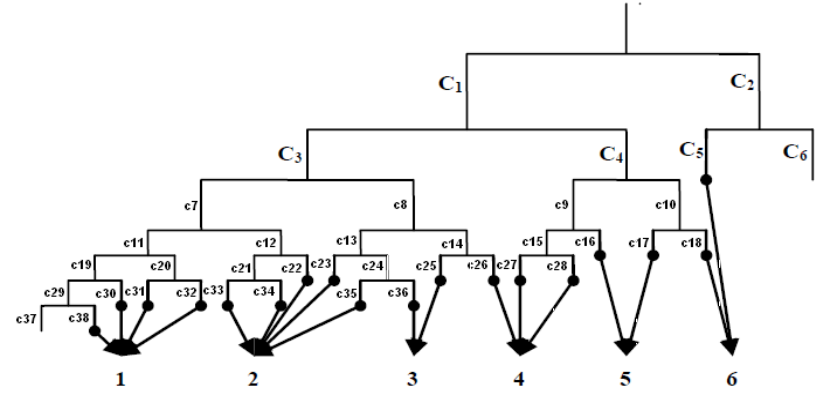
\includegraphics[width=\textwidth]{tree}
            \caption{Drzewo Dyskretnej transformaty pakietów falkowych}
            \label{fig:tree}
        \end{figure}
            
        \section{Podział sygnału na poszczególne pasma częstotliwości}
        \begin{itemize}
            \item \{0.39 - 3.13 Hz\}, Delta, współczynnik = [C38, C30, C31, C32]
            \item \{3.13 - 8.46 Hz\}, Theta, współczynnik = [C33, C34, C22, C23, C35]
            \item \{8.46 - 10.93 Hz\}, Alpha, współczynnik = [C36, C25]
            \item \{10.93 - 15.63 Hz\}, Spindle, współczynnik = [C26, C27, C28]
            \item \{15.63 - 21.88 Hz\}, Beta1, współczynnik = [C16, C17]
            \item \{21.88 - 37.50 Hz\}, Beta2, współczynnik = [C18, C5]         
        \end{itemize}

        \section{Cechy użyte do klasyfikacji sygnału}
        \begin{itemize}
            \item Średnie energie (E1, E2, E3, E4, E5, E6) współczynników reprezentujących każde z sześciu wymienionych wyżej pasm
            \item Całkowita energia (E7), która jest sumą energii wymienionych powyżej
            \item Stosunek energii pasma Alpha do sumy energii pasm Delta i Theta (E8)
            \item Stosunek energii pasma Delta do sumy energii pasm Alpha i Theta (E9)
            \item Stosunek energii pasma Theta do sumy energii pasm Delta i Alpha (E10)
            \item Średnia wartość współczynników we wszystkich pasmach
            \item Odchylenie standardowe współczynników we wszystkich pasmach
        \end{itemize}

    \chapter{Klasyfikacja faz snu w oparciu o sieć neuronową}

    %TODO
        normalizacja 
        struktura sieci
        uzyte funkcjonalnosci TensorFlow
        utworzone funkcje
        trenowanie
        wyniki, może w podsumowaniu

    \chapter*{Podsumowanie}
    \addcontentsline{toc}{chapter}{Podsumowanie}

    % \printbibliography[heading=bibintoc, title={Bibliografia}]

    \begin{appendices}
        \chapter{Pliki wykorzystane do treningu}
        \label{appendix:A}
        SC4001E0-PSG.edf \newline
        SC4002E0-PSG.edf \newline
        SC4011E0-PSG.edf \newline
        SC4012E0-PSG.edf \newline
        SC4021E0-PSG.edf \newline
        SC4022E0-PSG.edf \newline
        SC4031E0-PSG.edf \newline
        SC4032E0-PSG.edf \newline
        SC4041E0-PSG.edf \newline
        SC4042E0-PSG.edf \newline
        SC4051E0-PSG.edf \newline
        SC4052E0-PSG.edf \newline
        SC4061E0-PSG.edf \newline
        SC4062E0-PSG.edf \newline
        SC4071E0-PSG.edf \newline
        SC4072E0-PSG.edf \newline
        SC4081E0-PSG.edf \newline
        SC4082E0-PSG.edf \newline
        SC4091E0-PSG.edf \newline
        SC4092E0-PSG.edf \newline
        SC4122E0-PSG.edf \newline
        SC4131E0-PSG.edf \newline
        SC4141E0-PSG.edf \newline
        SC4142E0-PSG.edf \newline
        SC4151E0-PSG.edf \newline
        SC4152E0-PSG.edf \newline
        SC4161E0-PSG.edf

        \chapter{Pliki wykorzystane do testowania}
        \label{appendix:B}
        SC4101E0-PSG.edf \newline
        SC4102E0-PSG.edf \newline
        SC4111E0-PSG.edf \newline
        SC4112E0-PSG.edf \newline
        SC4121E0-PSG.edf

    \end{appendices}

\end{document}